\documentclass[12pt, a4paper]{article}
\addtolength{\oddsidemargin}{-.875in}
\addtolength{\evensidemargin}{-.875in}
\addtolength{\textwidth}{1.75in}
\addtolength{\topmargin}{-.875in}
\addtolength{\textheight}{1.75in}

\usepackage{indentfirst}
\usepackage{graphicx}
\usepackage{amsmath}


\begin{document}
\noindent
Nicholas Garrett\\ \\
Professor Griffith\\ \\
CS 3321\\ \\
10/22/2021\\ \\


\begin{center}
	\centering{	Homework 2\\ }
\end{center}

\noindent
1.
The three questions a Product Owner asks are: \\

What did you do since the last daily scrum?\\
	This is important so team members can know and determine how far along they are in the sprint.\\ 

What are your plans for the day?\\
	This is important to note to help motivate team members to maintain focus and complete required backlog items. \\ 

What is getting in the way of those plans?\\
	This question is important to help team members work as efficiently as possible \\ \\ \\

Two additional questions to ask:\\
	
How long do you think it will take to finish your tasks?\\
	This question helps team members to understand how much time will be required.\\

Have you identified any issues in the current sprint backlog? \\
	This question helps the team to determine if the current sprint is of a proper size. \\ \\ \\


2.\\
\indent
In the context of Essence, methods are compositions of practices that can be described by using Kernal elements.\\

Our team's method is fairly simple.  We use Scrum, especially its backlog, to maintain a working backlog of items to complete. We do a daily (weekly) standup to make sure we are all doing our tasks and working efficiently.  With our sprint meetings, where we discuss allocation and emphasis on the sprint, we determine how best to assign team members--e.g. for the first sprint, we split the team into frontend and backend to improve efficiency.
By assigning deadlines for which we are to have sprints--or even sub-sprints--completed, we try to work more efficiently.  \\ \\ \\

3.\\
Blackjack.\\

As a dealer, I need to make sure players put in at least the minimum bet so that the house can make money.
Given that there is a player and they make a bet, when their bet is below the minimum, then inform them they need to match the minimum bet or leave.

As a player, if I win, I need the return on my bet so the rules are followed.
Given that there is a player, and they have made a bet, when they win, then the player keeps their bet plus an equal amount from the dealer.

As a player, if I lose, I need to lose my money so the rules are followed.
Given that there is a player and they have made a bet, when they lose, then the player's bet is taken by the dealer.

As a player, if I get a blackjack, I need to get 1.5 times by bet from the dealer so the rules can be followed.
Given there is a player and they made a bet, when the get a blackjack, they win 1.5 times their bet from the dealer.

As a dealer, I need to shuffle the deck after every hand to ensure fairness.
Given there is a round and there is a deck of cards, when the round ends, shuffle the deck.

Some epics I found in this exercise were with regards to making the betting returns more specific.\\ \\ \\

4.

\begin{figure}[ht!]
\centering
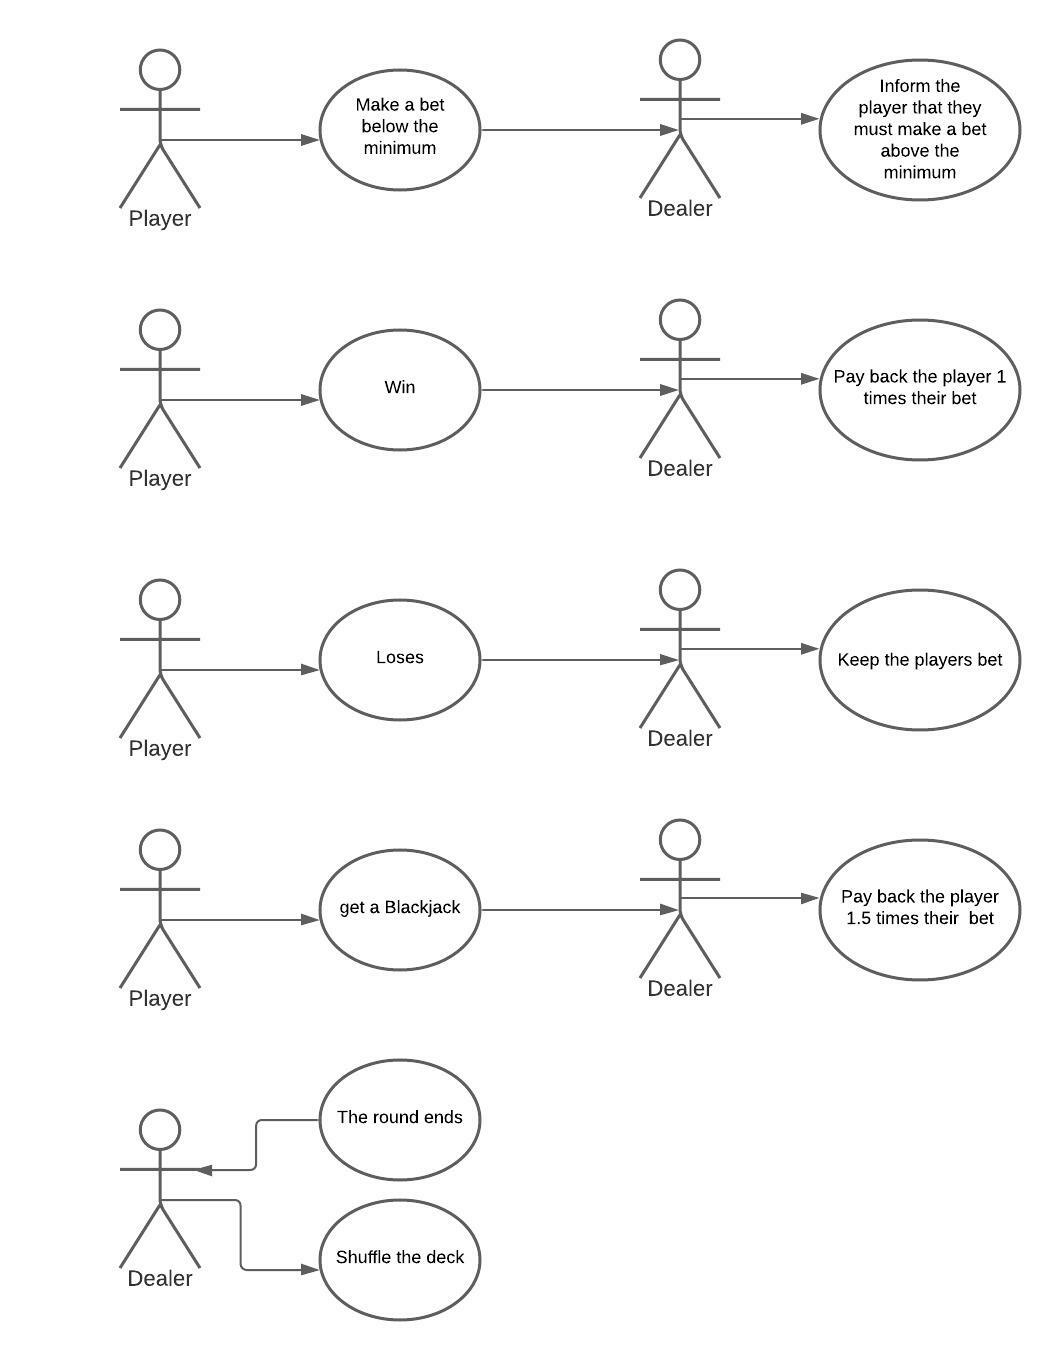
\includegraphics[width=90mm]{useCases.jpeg}
\end{figure}
First: This use case would probably take a couple of days to complete.\\
	
Second: This use case would probably take a few days to a week to complete due to the logic required to determine if a player had won or not.\\

Third: This use case would probably take a few days as well due to the logic required to determine if a player had won or not.\\

Fourth: This use case would most likely take only a few days as the logic only needs to check if the player has a Blackjack.\\

Fifth: This use case would probably take at least a week to implement, with the randomization and shuffling logic required.
\begin{figure}[ht!]
\centering
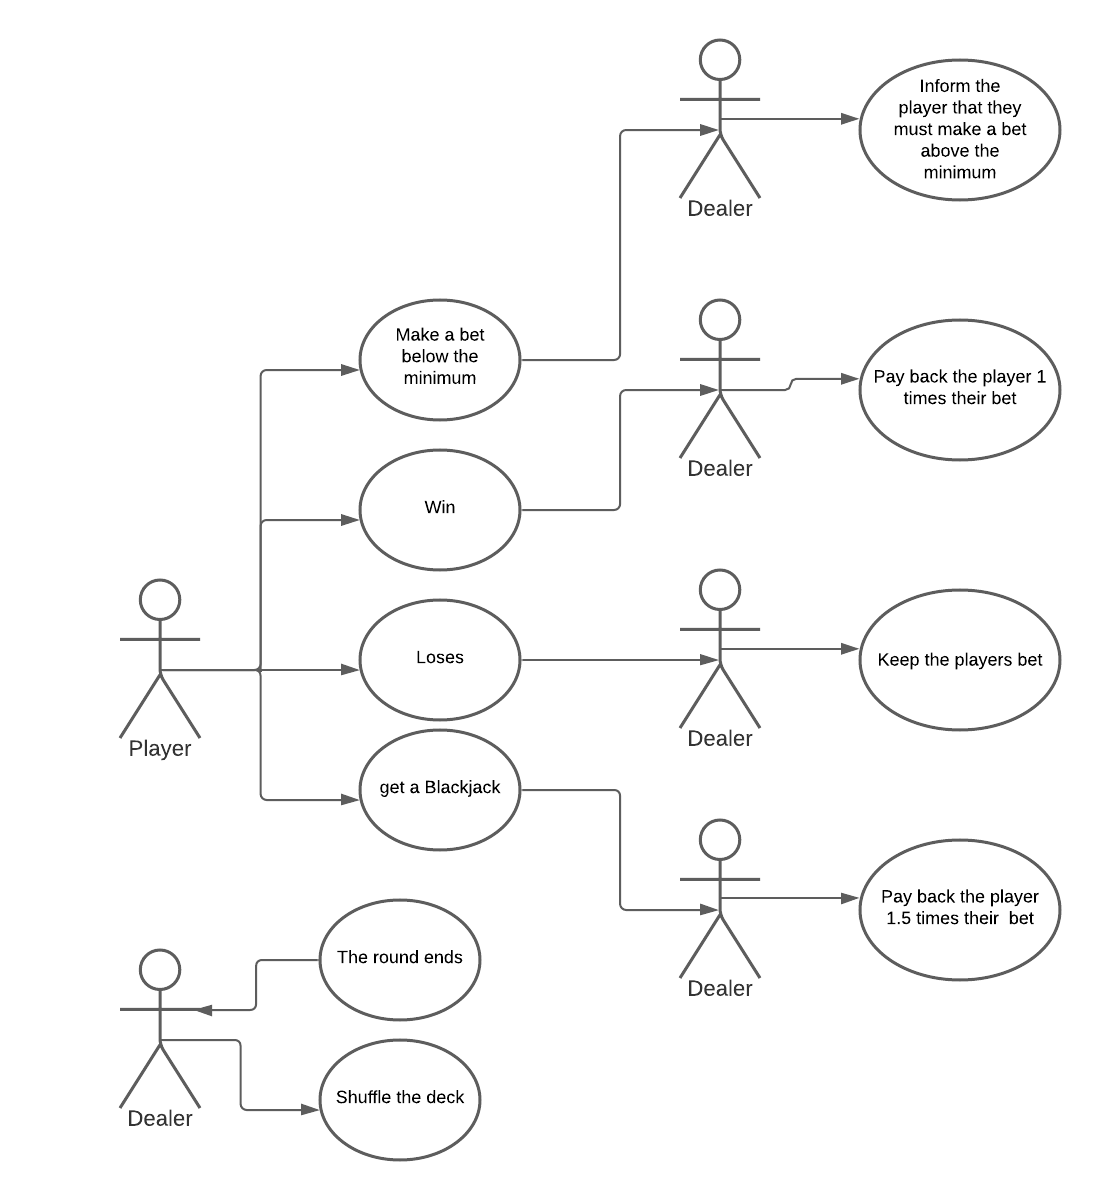
\includegraphics[width=90mm]{useCase.png}
\end{figure}.\\ \\ \\

5.\\

\begin{center}
Dealer
\begin{tabular}{ c || c  }
 Path & localhost:port/dealer  \\ 
 HTTP method &  GET and POST \\  
 Data format &  JSON    \\ 
Data to be sent/received & Card data, dealer's hand, bet data  \\ \\
\end{tabular}
\end{center}

\begin{center}
Player
\begin{tabular}{ c || c  }
 Path & localhost:port/player  \\ 
 HTTP method &  GET and POST \\  
 Data format &  JSON    \\
Data to be sent/received & card data, bet data,  \\ \\
\end{tabular}
\end{center}

\begin{center}
Deal Cards
\begin{tabular}{ c || c  }
 Path & localhost:port/deal  \\ 
 HTTP method &  POST \\  
 Data format &  JSON    \\
Data to be sent/received & Card data \\ \\
\end{tabular}
\end{center}

\begin{center}
Shuffle deck
\begin{tabular}{ c || c  }
 Path & localhost:port/shuffle  \\ 
 HTTP method &  GET and POST \\  
 Data format &  JSON    \\
Data to be sent/received & Card data \\ \\
\end{tabular}
\end{center}

\begin{center}
Determine if a winning hand
\begin{tabular}{ c || c  }
 Path & localhost:port/isWinningHand  \\ 
 HTTP method &  GET and POST \\  
 Data format &  JSON    \\
Data to be sent/received & card data and Boolean \\ \\
\end{tabular}
\end{center}

\begin{center}
Bet handler
\begin{tabular}{ c || c  }
 Path & localhost:port/bets  \\ 
 HTTP method &  GET and POST \\  
 Data format &  JSON    \\
Data to be sent/received & player bets \\ \\
\end{tabular}
\end{center}

\begin{figure}[ht!]
\centering
\includegraphics[width=90mm]{"blackjack UML.jpeg"}
\end{figure}


\end{document}  